% LaTeX template for reports
% Author: Adam Jaamour
% Last updated: 13/04/2020

% ------------------- IMPORTS -------------------
\documentclass[letterpaper,12pt]{article}
\usepackage{tabularx} % extra features for tabular environment
\usepackage{amsmath}  % improve maths presentation
\usepackage{amssymb} % maths symbols
\usepackage{graphicx} % takes care of graphic including machinery
\usepackage[margin=0.95in,letterpaper]{geometry} % decreases margins
\usepackage{cite} % takes care of citations
\usepackage[titletoc,title]{appendix} % takes care of appendices
\usepackage{listings} % code representation
\usepackage{pdflscape}
\usepackage{csquotes} % for quoting existing work
\usepackage{color} % defines colours for code listings
\usepackage{comment} % allows for block of comments
\usepackage{gensymb} % degree symbol
\usepackage[table,xcdraw]{xcolor} % table colouring
\usepackage[cc]{titlepic}  % allows a pic to be included in the title page
\usepackage[final]{hyperref} % adds hyper links inside the generated pdf file
\usepackage{pdfpages} % include pdfs

% ------------------- CODING STYLE -------------------
\definecolor{codegreen}{rgb}{0,0.6,0}
\definecolor{codegray}{rgb}{0.5,0.5,0.5}
\definecolor{backcolour}{rgb}{0.95,0.95,0.92}
\lstdefinestyle{mystyle}{
    backgroundcolor=\color{backcolour},   
    commentstyle=\color{codegreen},
    keywordstyle=\color{blue},
    numberstyle=\tiny\color{codegray},
    basicstyle=\footnotesize,
    breakatwhitespace=false,         
    breaklines=true,                 
    captionpos=b,                    
    keepspaces=true,                 
    numbersep=5pt,                  
    showspaces=false,                
    showstringspaces=false,
    showtabs=false,                  
    tabsize=4
}
\lstset{style=mystyle}

% ------------------- HEADINGS -------------------

\begin{document}

\title{
    (Main Title) Machine Learning\\ (Subtitle) Report\\
    \begin{large}
    (Organisation) University of St Andrews - School of Computer Science
    \end{large}
}
\titlepic{
\includegraphics[width=0.3\linewidth]{figures/st-andrews-logo.jpeg}}
\author{Adam Jaamour} % Student ID: 150014151
\date{7th May, 2020}
\maketitle
\newpage

\tableofcontents
\newpage

% ------------------- INTRODUCTION --------------------

\section{Introduction}
\label{sec:introduction}

Lorem ipsum dolor sit amet, consectetur adipiscing elit, sed do eiusmod tempor incididunt ut labore et dolore magna aliqua. Ut enim ad minim veniam, quis nostrud exercitation ullamco laboris nisi ut aliquip ex ea commodo consequat. Duis aute irure dolor in reprehenderit in voluptate velit esse cillum dolore eu fugiat nulla pariatur. Excepteur sint occaecat cupidatat non proident, sunt in culpa qui officia deserunt mollit anim id est laborum.\\

Content-Based Video Retrieval for Pattern Matching Video Clips \cite{Jaamour2019}.

% ------------------- PART 2: XXXX --------------------

\section{Section A}
\label{sec:section-A}

\subsection{Subsection i}

Egestas egestas fringilla phasellus faucibus scelerisque eleifend. Egestas sed sed risus pretium quam. Gravida neque convallis a cras semper auctor neque vitae. Posuere urna nec tincidunt praesent. Viverra ipsum nunc aliquet bibendum enim facilisis gravida neque convallis. Nisi est sit amet facilisis magna etiam tempor. Risus feugiat in ante metus. Velit egestas dui id ornare. Porttitor lacus luctus accumsan tortor posuere ac ut consequat.\\

Semper risus in hendrerit gravida rutrum quisque non tellus. Quis vel eros donec ac. Nulla at volutpat diam ut venenatis tellus in metus vulputate. Eleifend donec pretium vulputate sapien nec sagittis aliquam malesuada bibendum. Tellus at urna condimentum mattis pellentesque id nibh tortor. Dignissim enim sit amet venenatis urna. Cras semper auctor neque vitae tempus quam pellentesque. Egestas erat imperdiet sed euismod nisi porta lorem mollis.

\subsection{Subsection ii}

Vestibulum rhoncus est pellentesque elit ullamcorper. Eleifend donec pretium vulputate sapien nec. Risus quis varius quam quisque id diam vel quam elementum. Commodo sed egestas egestas fringilla phasellus. Sed egestas egestas fringilla phasellus faucibus scelerisque eleifend. Non curabitur gravida arcu ac tortor dignissim. Eu consequat ac felis donec. Aliquet lectus proin nibh nisl condimentum id venenatis a. Tortor vitae purus faucibus ornare suspendisse sed nisi lacus. Commodo nulla facilisi nullam vehicula ipsum.

% ------------------- PART 3: XXXX --------------------

\section{Section B}
\label{sec:section-B}

In mollis nunc sed id. Ligula ullamcorper malesuada proin libero nunc consequat interdum varius sit. Consequat id porta nibh venenatis cras sed felis. Sed adipiscing diam donec adipiscing tristique risus. Elit duis tristique sollicitudin nibh sit amet. In tellus integer feugiat scelerisque varius morbi enim nunc. Habitant morbi tristique senectus et. Tincidunt tortor aliquam nulla facilisi cras fermentum odio. Id volutpat lacus laoreet non. Sapien et ligula ullamcorper malesuada proin libero nunc consequat interdum. Quisque id diam vel quam elementum. Nulla facilisi cras fermentum odio eu feugiat. Eget felis eget nunc lobortis mattis aliquam faucibus purus. Elit eget gravida cum sociis.

% ------------------- CONCLUSION --------------------

\section{Conclusion}
\label{sec:conclusion}

Cum sociis natoque penatibus et magnis dis. Odio aenean sed adipiscing diam donec. Bibendum enim facilisis gravida neque convallis a cras. Ligula ullamcorper malesuada proin libero. Libero nunc consequat interdum varius sit amet. Vitae auctor eu augue ut lectus. Metus aliquam eleifend mi in nulla posuere sollicitudin aliquam ultrices. Cursus eget nunc scelerisque viverra mauris in aliquam. Pulvinar sapien et ligula ullamcorper malesuada proin libero nunc consequat.\\

Leo urna molestie at elementum. Aliquam sem et tortor consequat id porta. Ac turpis egestas sed tempus urna. At erat pellentesque adipiscing commodo elit at imperdiet dui accumsan. Bibendum at varius vel pharetra vel turpis. Nec feugiat nisl pretium fusce id velit ut tortor pretium. Leo urna molestie at elementum eu facilisis. Enim ut tellus elementum sagittis vitae. Scelerisque eleifend donec pretium vulputate sapien.


% -------------------- APPENDIX --------------------

\begin{appendices}

\clearpage

\bibliographystyle{plain}
\bibliography{bibliography}

% --------------------

\clearpage
\section{Demo Figure}
\label{sec:appendix-demo-figure}

\begin{figure}[h]
\centerline{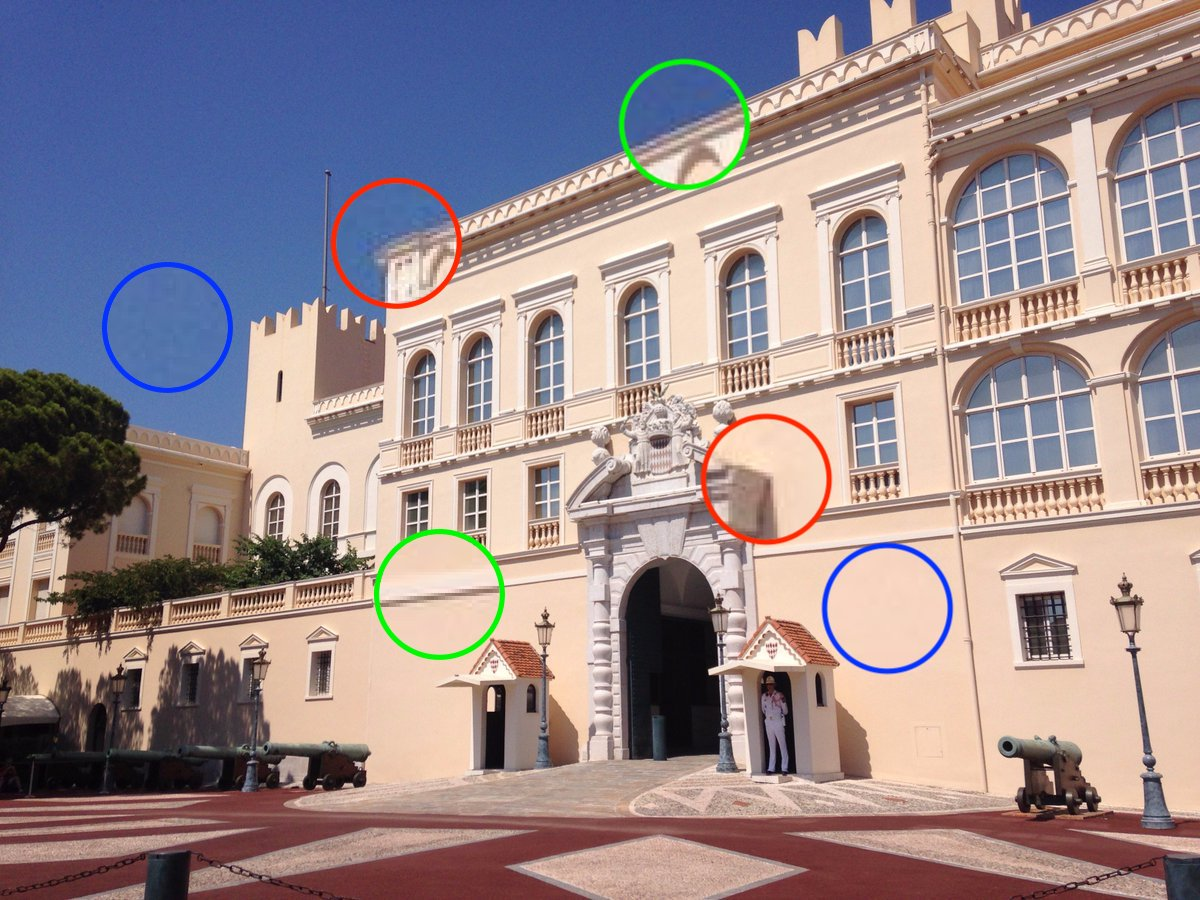
\includegraphics[width=0.95\textwidth]{figures/demo_figure.jpg}}
\caption{\label{fig:demo_figure}Potential points of interest for dynamic features (blue = flat, green = edges, red = corners).}
\end{figure}

% --------------------

\clearpage
\section{Demo Table}
\label{sec:appendix-demo-table}

\begin{table}[h]
\centering
\begin{tabular}{lll}
A & B  & C   \\
1 & 2  & 3   \\
I & II & III
\end{tabular}
\caption{Demo table}
\label{tab:my-table}
\end{table}

% ------------------------

\end{appendices}
\end{document}